%%%%%%%%%%%%%%%%%%%%%%%%%%%%%%%%%%%%%%%%%%%%%%%%%%%%%%%%%%%%%%%%%%%%%%%%%%
%%
%%	Author Submission Template for Operations Research (OPRE)
%%	INFORMS, <informs@informs.org>
%%	Ver. 1.00, June 2024
%%  Modified by Jiheng Zhang @ UST
%%
%%%%%%%%%%%%%%%%%%%%%%%%%%%%%%%%%%%%%%%%%%%%%%%%%%%%%%%%%%%%%%%%%%%%%%%%%%
%
% Use dblanonrev for Double Anonymous Review submission
% Use sglanonrev for Single Anonymous Review submission
% For example, submission to INFORMS Mathematics of Operation Research, MOOR will have
% \documentclass[moor,dblanonrev]{style/informs4}
%
% \documentclass[opre,dblanonrev]{style/informs4}
\makeatletter
\def\input@path{{style/}}  % 告诉 LaTeX 在 style/ 目录下搜索文件
\makeatother
\documentclass[opre,sglanonrev]{informs4}


% \usepackage{amsthm} % 引入 amsthm 包以支持 newtheorem
\newtheorem{policy}{Policy}

% \usepackage{eqndefns-left} % For checking the display equation width and equation environment definitions %
\bibliographystyle{style/informs2014}
\usepackage{natbib}
 \bibpunct[, ]{(}{)}{,}{a}{}{,}%
 \def\bibfont{\small}%
 \def\bibsep{\smallskipamount}%
 \def\bibhang{24pt}%
 \def\newblock{\ }%
 \def\BIBand{and}%

\input{style/formality.tex}
\input{tikz/setting.tex}

% Load the fix-cm package
\usepackage{fix-cm}
% Manually declare missing font shapes if necessary
\DeclareFontShape{OML}{cmm}{b}{it}{<->cmmib10}{}
\DeclareFontShape{OMS}{cmsy}{b}{n}{<->cmsy10}{}

%\OneAndAHalfSpacedXI
\OneAndAHalfSpacedXII % Current default line spacing
%%\DoubleSpacedXI
%%\DoubleSpacedXII

%% Setup of the equation numbering system. Outcomment only one.
%% Preferred default is the first option.
\EquationsNumberedThrough    % Default: (1), (2), ...
%\EquationsNumberedBySection % (1.1), (1.2), ...

%% Setup of theorem styles. Outcomment only one.
%% Preferred default is the first option.
\TheoremsNumberedThrough     % Preferred (Theorem 1, Lemma 1, Theorem 2)
%\TheoremsNumberedByChapter  % (Theorem 1.1, Lema 1.1, Theorem 1.2)
\ECRepeatTheorems  %  

% For new submissions, leave this number blank.
% For revisions, input the manuscript number assigned by the on-line
% system along with a suffix ".Rx" where x is the revision number.
% \MANUSCRIPTNO{MOOR-0001-2024.00}

%%%%%%%%%%%%%%%%
\begin{document}
%%%%%%%%%%%%%%%%

% Outcomment only when entries are known. Otherwise leave as is and
%   default values will be used.
%\setcounter{page}{1}
%\VOLUME{00}%
%\NO{0}%
%\MONTH{Xxxxx}% (month or a similar seasonal id)
%\YEAR{0000}% e.g., 2005
%\FIRSTPAGE{000}%
%\LASTPAGE{000}%
%\SHORTYEAR{00}% shortened year (two-digit)
%\ISSUE{0000} %
%\LONGFIRSTPAGE{0001} %
%\DOI{10.1287/xxxx.0000.0000}%

% Author's names for the running heads
% Sample depending on the number of authors;
% \RUNAUTHOR{Jones}
% \RUNAUTHOR{Jones and Wilson}
% \RUNAUTHOR{Jones, Miller, and Wilson}
% \RUNAUTHOR{Jones et al.} % for four or more authors
% Enter authors following the given pattern:
%\RUNAUTHOR{}

% Title or shortened title suitable for running heads. Sample:
% \RUNTITLE{}

% Enter the full title:
\TITLE{Airline Cargo Transport Recovery}

\ARTICLEAUTHORS{%
%\AUTHOR{John Doe,\textsuperscript{a} Jane Smith,\textsuperscript{b}}
%\AFF{\textsuperscript{a}Department of Industrial Engineering, University of XYZ, \EMAIL{john.doe@xyz.edu; \textsuperscript{b}Department of Computer Science, University of ABC, \EMAIL{jane.smith@abc.edu}} 
% Enter all authors
}

\ABSTRACT{
    % big background
    Stochastic. 
    % what is novel
    However, .
    % what is our model
    Specifically, .
    % What we do (challenge, results, methodology)
    .
    % Numerical experiments
    Numerical experiments.
}%

%\FUNDING{This research was supported by [grant number, funding agency].}

\KEYWORDS{Stochastic control, Queueing network,Uncertainty, Online learning, Optimization} 

%\HISTORY{Received: Month DD, YYYY; Accepted: Month DD, YYYY; Published Online: Month DD, YYYY}

\maketitle
%%%%%%%%%%%%%%%%%%%%%%%%%%%%%%%%%%%%%%%%%%%%%%%%%%%%%%%%%%%%%%%%%%%%%%

% Text of your paper here
\section{Introduction}
%Motivation
waiting costs.
Unlike passengers, cargo from the same batch does not experience dissatisfaction or request refunds %
due to reassignment to direct or connecting flights. Therefore, this model employs a narrative based on cargo %
accumulation and passenger aircraft bellyhold recovery. 
%Real world 

\cite{Erlang1948,Dantzig1955,Dynkin1956,Bellman1957DP,Little1961,Skorokhod1961,McKean1965,Iglehart1965}

\section{Literature Review}

\section{Situation of a single Backlog point}
In this section, we will find out how to design a recovery plan for cargo transport under ideal (static) conditions in Section 3.2. Considering that in actual (dynamic) situations with randomness, applying the policy from the static case may lead to deviations, the dynamic situation is discussed in Section 3.3. At this point, if there is ample remaining space on direct flights during a certain period, it may happen that transfer flights arrive but are not used, in which case the optimal dynamic decision may differ from the deterministic decision.

\subsection{Basic Settings}
\label{sec:basic_settings}


\subsubsection{Backlog}
At the original airport, due to factors such as flight cancellations, a total of \( B \) units of cargo cannot be transported as initially scheduled. These cargos are randomly organized into a queue, waiting for transfer to the available capacity of subsequent flights to reach their intended destinations.

\subsubsection{Service}
Upon arrival, each cargo unit can be assigned to one of two types of servers, Direct or Transfer, each with a total capacity of \( R \).

\begin{itemize}
    \item \textbf{Direct flights (Direct server):} Direct flights from the original airport directly to the destination airport. Interdeparture times follow an exponential distribution \( I \sim \text{Exp}(\mu_0) \), indicating that direct flight departures form a Poisson process with a rate of \( \mu_0 \). The residual load rate available for each direct flight, denoted \( C_0(t) \sim U(0,1] \), determines the capacity to transport backlog cargo, the actual available cargo capacity being \( R \cdot C_0(t) \). Only one Direct server can depart at a time. When the cargo backlog is substantial, multiple Direct servers may be required, resulting in potential waiting times for some cargo units.
    
    \item \textbf{Transfer flights (Transfer server):} Transfer flights operate from the original airport to the destination airport via a designated transfer airport. The departure of transfer flights follows a Poisson process with a rate of \( \mu_1 \). We consider only a single transfer scenario, where the transfer airport could be one of several possible cities, denoted \( A_1, A_2, \ldots, A_n \). The available residual load rate for each transfer flight is \( C_1(t) \sim U(0,1] \), resulting in a actual cargo capacity of \( R \cdot C_1(t) \). The transfer time is modeled as a random variable \( X \), with an expected value of \( E(X) \).
\end{itemize}

\subsection{Model under Static Condition}
\label{sec:static_model}
%%%%%%%%%%%%%%%%%% Model-Dual
In conventional logistics planning, direct flights are generally prioritized for cargo transportation due to their inherent time efficiency, as they eliminate transfer waiting periods. This operational preference naturally leads to the establishment of a queueing principle: cargos positioned at the front of the queue should be loaded onto available direct flights immediately, with priority given to awaiting direct flight capacity when feasible. However, the principle may be counterproductive for cargos positioned toward the end of the queue, where prolonged waiting for direct flights could paradoxically result in later arrival times at destination compared to immediate transfer routing, as demonstrated in Figure~1.
%%%%%%%%%%% Figure 1

\begin{figure}[htbp]
    \centering
    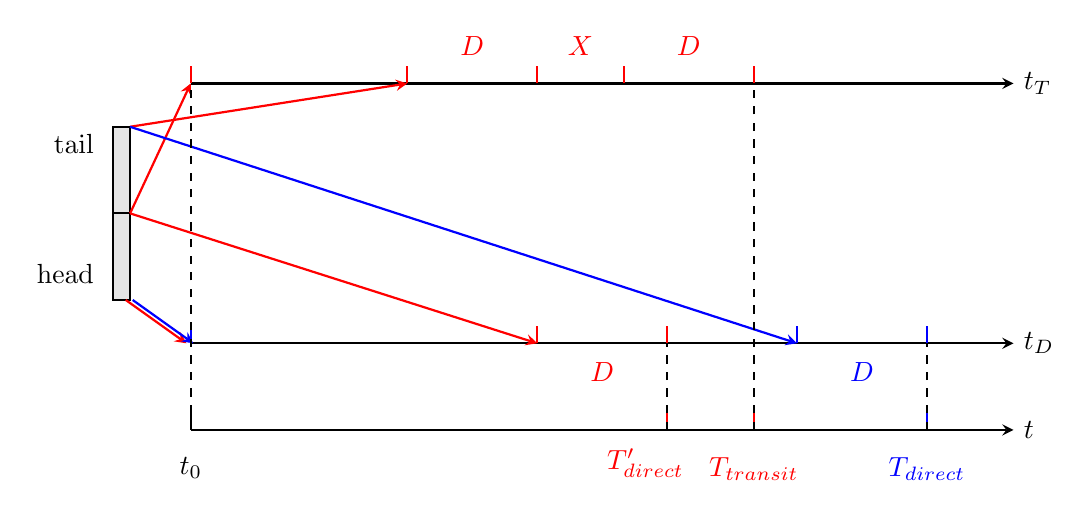
\begin{tikzpicture}[>=stealth, thick, scale=1.1]
        % Axes
        \draw[->] (0.5,3) -- (10,3) node[right] {$t_T$};
        \draw[->] (0.5,0) -- (10,0) node[right] {$t_D$};
        \draw[->] (0.5,-1) -- (10,-1) node[right] {$t$};
        % Y labels
        \node[left] at (-0.5,2.3) {tail};
        \node[left] at (-0.5,0.8) {head};
        % Vertical bar for queue
        \draw[fill=gray!20] (-0.4,0.5) rectangle (-0.2,2.5);
        % Horizontal lines for queue
        \draw (-0.4,1.5) -- (-0.2,1.5);
        % Arrows from queue to time axis
        \draw[->,red] (-0.2,2.5) -- (3,3);
        \draw[->,red] (-0.2,1.5) -- (0.5,3);
        \draw[->,red] (-0.2,1.5) -- (4.5,0);
        \draw[->,red] (-0.25,0.5) -- (0.45,0);
        \draw[->,blue] (-0.2,2.5) -- (7.5,0);
        \draw[->,blue] (-0.17,0.5) -- (0.53,0);
        % markers_Transit
        \draw[red] (0.5,3) -- (0.5,3.2);
        \draw[red] (3,3) -- (3,3.2);
        \draw[red] (4.5,3) -- (4.5,3.2);
        \draw[red] (5.5,3) -- (5.5,3.2);
        \draw[red] (7,3) -- (7,3.2);
        % Labels_Transit
        \node[above, text=red] at (3.75,3.2) {$D$};
        \node[above, text=red] at (5,3.2) {$X$};
        \node[above, text=red] at (6.25,3.2) {$D$};
        % markers_Direct
        \draw[blue] (0.5,0) -- (0.5,0.2);
        \draw[red] (4.5,0) -- (4.5,0.2);
        \draw[red] (6,0) -- (6,0.2);
        \draw[blue] (7.5,0) -- (7.5,0.2);
        \draw[blue] (9,0) -- (9,0.2);
        % Labels_Direct
        \node[below, text=blue] at (8.25,-0.1) {$D$};
        % Labels_Direct'
        \node[below, text=red] at (5.25,-0.1) {$D$};
        % markers_t
        \draw[black] (0.5,-1) -- (0.5,-0.8);
        \draw[red] (6,-1) -- (6,-0.8);
        \draw[red] (7,-1) -- (7,-0.8);
        \draw[blue] (9,-1) -- (9,-0.8);
        % Labels_t
        \node[below] at (0.5,-1.2) {$t_0$};
        \node[below,red] at (7,-1.2) {$T_{transit}$};
        \node[below,blue] at (9,-1.2) {$T_{direct}$};
        \node[below,red] at (5.75,-1.1) {$T_{direct}'$};
        % Time markers 
        \draw[dashed] (0.5,-1) -- (0.5,3);
        % \draw[dashed] (4.5,-1) -- (4.5,0);
        \draw[dashed] (6,-1) -- (6,0);
        \draw[dashed] (7,-1) -- (7,3);
        \draw[dashed] (9,-1) -- (9,0);
    \end{tikzpicture}
    \caption{Illustration of cargo assignment and waiting times for direct and transfer flights.}
    \label{fig:mix_waiting}
\end{figure}

The disrupted cargos randomly line up in a queue without discrimination, %
as illustrated by the gray rectangle on the left side of Figure 1, the constraints %
imposed by $C_0$ and $C_1$ dictate a sequential order for the recovery process. %
Subsequent flights commence from the head of the queue and continue until the final %
unit of cargo at the tail of the queue is transported, thereby completing the recovery %
task for this segment. From a practical perspective, decision-makers are inclined to %
prioritize a strategy where disrupted cargo awaits direct flights, as depicted by the blue %
arrows in Figure 1, representing the all-direct recovery scheme. The temporal composition %
of this recovery process is reflected along the $t_D$ axis. For simplicity, we approximate %
the flight transportation time as a constant $D$. The recovery process concludes once the %
final unit of cargo reaches its destination. However, such an all-direct strategy may result %
in excessively prolonged waiting times for cargo at the tail of the queue. An alternative %
approach involves arranging a portion of the disrupted cargo for transfer flights at the %
outset of the recovery period, as illustrated by the red arrows in Figure 1, representing %
the hybrid recovery scheme. At the start of the recovery period, the random queue is %
immediately segmented, with part of the cargo following the all-direct recovery strategy %
and the remainder utilizing transfer flights. The temporal composition of the recovery %
process for transfer flights is reflected along the $t_T$ axis. If the waiting cost for %
cargo in the time interval from $T_{\text{direct}}'$ to $T_{\text{direct}}$ exceeds the %
waiting cost for cargo in the time interval from $t_0$ to $T_{\text{transit}}$, the hybrid %
recovery strategy may prove more advantageous.

To address the challenge of temporal optimization, we propose a cargo segmentation model with capacity-aware temporal thresholds. We assume that selecting direct or transfer flights for durations of \(0 - T_0\) or \(0 - T_1\), respectively, fully utilizes the available residual capacities of the flights (\(C_0(t)\) and \(C_1(t)\)) during these periods. In this way, cargo waiting times are effectively managed on direct and transfer flights.

\begin{itemize}
    \item \textbf{Direct Flight Threshold ($T_0$)}: Defines the time period $[0, T_0]$ during which waiting cargoes can await direct flight availability. The residual capacity of direct flights at time $t$ within this period, denoted $C_0(t)$, is fully utilized through continuous loading operations.
    
    \item \textbf{Transfer Flight Threshold ($T_1$)}: Specifies the maximum waiting duration $[0, T_1]$ for the transfer flight allocation. Similarly to direct flights, all transfer capacity available $C_1(t)$ within this interval is completely occupied.
\end{itemize}

% Defining the objective function
The objective function is given by:
\[ T_w = \int_{0}^{T_0} R C_0(t) t \, dt + \int_{0}^{T_1} R C_1(t) (t + X) \, dt \]

% Explaining the objective function
The function calculates the product of the waiting time from transportation interruption to re-transportation and the amount of that batch of cargos waiting for direct flights or transfer flights, respectively. We evaluate the quality of the plan by the waiting cost \( T_w \), optimizing the values of \( T_0 \) and \( T_1 \) to minimize \( T_w \). The expected waiting cost, incorporating the flight arrival rates \(\mu_0\) for direct flights and \(\mu_1\) for transfer flights, is:
\[ E[T_w] = E\left[ \int_{0}^{T_0} R C_0(t) t \, dt \right] + E\left[ \int_{0}^{T_1} R C_1(t) (t + X) \, dt \right] = \frac{R \mu_0}{4} T_0^2 + \frac{R \mu_1}{4} T_1^2 + \frac{R \mu_1}{2} E[X] T_1 \]

% Specifying the cargo backlog constraint
Furthermore, the sum of the amount of cargo transported by direct flights and by transfer flights should equal the total cargo backlog, which means that all disrupted cargo must be fully transported:
\[ \int_{0}^{T_0} R C_0(t) \, dt + \int_{0}^{T_1} R C_1(t) \, dt = B \]

% Calculating the expected value of transported cargo
The expected value, which accounts for the flight arrival frequencies, is:
\[ E\left[ \int_{0}^{T_0} R C_0(t) \, dt + \int_{0}^{T_1} R C_1(t) \, dt \right] = \frac{R \mu_0}{2} T_0 + \frac{R \mu_1}{2} T_1 \]

Then, our optimization problem can be defined as follows:
\begin{align*}
\min_{T_0, T_1} \quad & \frac{R \mu_0}{4} T_0^2 + \frac{R \mu_1}{4} T_1^2 + \frac{R \mu_1 E[X]}{2} T_1 \\
\text{s.t.} \quad & \frac{R}{2} (\mu_0 T_0 + \mu_1 T_1) = B \\
& T_0 \geq 0
\quad T_1 \geq 0
\end{align*}


% Presenting the updated optimal policy
\begin{theorem}
	\label{thm:optimal_policy}
    As long as the cargo backlog \( B \), flight capacity \( R \), expected transfer time \( E[X] \), and flight arrival rates \(\mu_0\) and \(\mu_1\) satisfy the optimization problem, the optimal waiting time thresholds \( T_0 \) and \( T_1 \) are given by: \begin{itemize}
        \item If \( B \geq \frac{R \mu_0}{2} E[X] \):
        \[
        T_0 = \frac{\frac{2B}{R} + \mu_1 E[X]}{\mu_0 + \mu_1}, \quad T_1 = \frac{\frac{2B}{R} - \mu_0 E[X]}{\mu_0 + \mu_1}
        \]
        \item If \( B < \frac{R \mu_0}{2} E[X] \):
        \[
        T_0 = \frac{2B}{R \mu_0}, \quad T_1 = 0
        \]
    \end{itemize}
\end{theorem}

% Providing the updated proof
\begin{proof}{Proof of Theorem~\ref{thm:optimal_policy}}
The optimal waiting-time thresholds are derived using the Lagrangian dual method. Construct the Lagrangian function based on the optimization problem:

\[
L(T_0, T_1, \lambda) = \frac{R \mu_0}{4} T_0^2 + \frac{R \mu_1}{4} T_1^2 + \frac{R \mu_1}{2} E[X] T_1 + \lambda \left( B - \frac{R \mu_0}{2} T_0 - \frac{R \mu_1}{2} T_1 \right)
\]
where \( \lambda \) is the Lagrange multiplier that represents the marginal cost per unit of cargo.

% Defining the dual function
The dual function is the infimum of the Lagrangian over \( T_0 \) and \( T_1 \), considering non-negativity constraints:
\[
g(\lambda) = \inf_{T_0 \geq 0, T_1 \geq 0} L(T_0, T_1, \lambda)
\]

% Computing partial derivatives
To find \( g(\lambda) \), compute the partial derivatives of \( L \):
\[
\frac{\partial L}{\partial T_0} = \frac{R \mu_0}{2} T_0 - \frac{R \mu_0}{2} \lambda = 0 \implies T_0 = \lambda
\]
Since \( T_0 \geq 0 \), we require \( \lambda \geq 0 \).
\[
\frac{\partial L}{\partial T_1} = \frac{R \mu_1}{2} T_1 + \frac{R \mu_1}{2} E[X] - \frac{R \mu_1}{2} \lambda = 0 \implies T_1 = \lambda - E[X]
\]
Since \( T_1 \geq 0 \), we require \( \lambda \geq E[X] \). If \( \lambda < E[X] \), set \( T_1 = 0 \).

% Analyzing cases based on lambda
We analyze two cases based on the value of \( \lambda \):

% Case 1: lambda >= E[X]
\textbf{Case 1: \( \lambda \geq E[X] \)} \\
Set:
\[
T_0 = \lambda, \quad T_1 = \lambda - E[X]
\]
Substitute in the constraint:
\[
\frac{R \mu_0}{2} \lambda + \frac{R \mu_1}{2} (\lambda - E[X]) = B
\]
\[
\frac{R}{2} \left( (\mu_0 + \mu_1) \lambda - \mu_1 E[X] \right) = B
\]
\[
(\mu_0 + \mu_1) \lambda - \mu_1 E[X] = \frac{2B}{R}
\]
\[
\lambda = \frac{\frac{2B}{R} + \mu_1 E[X]}{\mu_0 + \mu_1}
\]
Thus:
\[
T_0 = \lambda = \frac{\frac{2B}{R} + \mu_1 E[X]}{\mu_0 + \mu_1}, \quad T_1 = \lambda - E[X] = \frac{\frac{2B}{R} - \mu_0 E[X]}{\mu_0 + \mu_1}
\]
Verify the condition for \( T_1 \geq 0 \):
\[
\frac{\frac{2B}{R} - \mu_0 E[X]}{\mu_0 + \mu_1} \geq 0 \implies \frac{2B}{R} \geq \mu_0 E[X] \implies B \geq \frac{R \mu_0}{2} E[X]
\]
This matches the condition for Case 1.

% Case 2: 0 <= lambda < E[X]
\textbf{Case 2: \( 0 \leq \lambda < E[X] \)} \\
Since \( T_1 = \lambda - E[X] < 0 \), set \( T_1 = 0 \), and \( T_0 = \lambda \). Substitute in the constraint:
\[
\frac{R \mu_0}{2} T_0 + \frac{R \mu_1}{2} \cdot 0 = B \implies \frac{R \mu_0}{2} T_0 = B \implies T_0 = \frac{2B}{R \mu_0}
\]
Then:
\[
\lambda = T_0 = \frac{2B}{R \mu_0}
\]
Check if \( \lambda < E[X] \):
\[
\frac{2B}{R \mu_0} < E[X] \implies B < \frac{R \mu_0}{2} E[X]
\]
This matches the condition for Case 2.

% Verifying the original constraint
We verify that the solutions satisfy the original constraint \( \frac{R \mu_0}{2} T_0 + \frac{R \mu_1}{2} T_1 = B \):

% Case 1 verification
For \( B \geq \frac{R \mu_0}{2} E[X] \):
\[
\frac{R \mu_0}{2} T_0 + \frac{R \mu_1}{2} T_1 = \frac{R \mu_0}{2} \cdot \frac{\frac{2B}{R} + \mu_1 E[X]}{\mu_0 + \mu_1} + \frac{R \mu_1}{2} \cdot \frac{\frac{2B}{R} - \mu_0 E[X]}{\mu_0 + \mu_1}
\]
\[
= \frac{R}{2} \cdot \frac{\mu_0 \left( \frac{2B}{R} + \mu_1 E[X] \right) + \mu_1 \left( \frac{2B}{R} - \mu_0 E[X] \right)}{\mu_0 + \mu_1}
\]
\[
= \frac{R}{2} \cdot \frac{\mu_0 \frac{2B}{R} + \mu_0 \mu_1 E[X] + \mu_1 \frac{2B}{R} - \mu_1 \mu_0 E[X]}{\mu_0 + \mu_1} = \frac{R}{2} \cdot \frac{(\mu_0 + \mu_1) \frac{2B}{R}}{\mu_0 + \mu_1} = \frac{R}{2} \cdot \frac{2B}{R} = B
\]
The constraint is satisfied, and \( T_0 \geq 0 \), \( T_1 \geq 0 \).

% Case 2 verification
For \( B < \frac{R \mu_0}{2} E[X] \):
\[
\frac{R \mu_0}{2} T_0 + \frac{R \mu_1}{2} T_1 = \frac{R \mu_0}{2} \cdot \frac{2B}{R \mu_0} + \frac{R \mu_1}{2} \cdot 0 = B + 0 = B
\]
The constraint is satisfied and \( \lambda = \frac{2B}{R \mu_0} < E[X] \), which is consistent.

% Deriving the optimal policy
The optimal policy is derived from the values of \( \lambda \):
\begin{itemize}
    \item When \( B \geq \frac{R \mu_0}{2} E[X] \), use both direct and transfer flights.
    \item When \( B < \frac{R \mu_0}{2} E[X] \), use only direct flights, as the lag does not justify the additional transfer time.
\end{itemize}
\end{proof}

%%%%%%%%%%%%%%%%%%%%%%%%%%%%%%%%%%%%%%%
%%%%%%%%%%%%%%%%%%%%%%%%%%%%%%%%%%%%%%% deter DP Model
\subsection{deterministic DP model}

From a dynamic programming perspective, let \( t \) denote the time elapsed since accumulation, \( b \) represent the remaining cargo backlog, and \( (b, t) \) define the state. We designate \( x_0 \) (cargo transported by direct flights) and \( x_1 \) (cargo transported by transfer flights) as the decision variables in state \( (b, t) \).
%%%%%%%%%%%%%%%%%%%%%%%%%%%%%%%%%%%%%%% Theorem 2
\begin{theorem}
\label{thm:optimal_policy_dp}
The optimal policy for decision variables \( x_0 \) and \( x_1 \) in state \( (b, t) \) is:
\begin{itemize}
    \item If \( b \geq \mu_0 R (t + E[X]) \):
    \[
    x_0 = \min(b, 0.5R), \quad x_1 = \min(b, 0.5R)
    \]
    \item If \( b < \mu_0 R (t + E[X]) \):
    \[
    x_0 = \min(b, 0.5R), \quad x_1 = 0
    \]
\end{itemize}
\end{theorem}

\begin{proof}{Proof of Theorem~\ref{thm:optimal_policy_dp}}

The state is \( (b, t) \), where \( b \) is the remaining cargo backlog and \( t \) is the time since accumulation. The value function \( V(b, t) \) is the minimum expected waiting cost, governed by:
\[
V(b, t) = \left\{
\begin{array}{l}
(1 - (\mu_0 + \mu_1) \Delta t) \left[ V(b, t + \Delta t) + b \cdot \Delta t \right] \\
+ \mu_0 \Delta t \cdot \left[ \min_{0 \leq x_0 \leq \min(b, 0.5R)} \left( V(b - x_0, t + \Delta t) + x_0 \cdot t \right) \right] \\
+ \mu_1 \Delta t \cdot \left[ \min_{0 \leq x_1 \leq \min(b, 0.5R)} \left( V(b - x_1, t + \Delta t) + x_1 \cdot (t + E[X]) \right) \right]
\end{array}
\right\}
\]
Direct flights arrive at rate \( \mu_0 \), transfer flights at rate \( \mu_1 \), each with capacity \( 0.5R \), and transfer flights incur an additional delay \( E[X] \).

% Step 1: Hypothesize value function
Consider the terms:
\[
V(b, t) = b \cdot w(t)
\]
where \( w(t) \) is the marginal waiting cost per unit of cargo. This is motivated by the linear cost structure (\( b \cdot \Delta t \), \( x_0 \cdot t \), \( x_1 \cdot (t + E[X]) \)).

% Step 2: Analyze minimization terms
Substitute \( V(b, t) = b w(t) \) into the Bellman equation:
\begin{itemize}
    \item \textbf{Waiting term}:
    \[
    V(b, t + \Delta t) + b \cdot \Delta t
    \]
    Represents the cost of keeping \( b \) units waiting for \( \Delta t \).
    \item \textbf{Direct flight term}:
    \[
    \min_{0 \leq x_0 \leq \min(b, 0.5R)} \left[ V(b - x_0, t + \Delta t) + x_0 \cdot t \right]
    \]
    The cost of transporting \( x_0 \) units via direct flights at time \( t \).
    \item \textbf{Transfer flight term}:
    \[
    \min_{0 \leq x_1 \leq \min(b, 0.5R)} \left[ V(b - x_1, t + \Delta t) + x_1 \cdot (t + E[X]) \right]
    \]
    The cost of transporting \( x_1 \) units via transfer flights, including delay \( E[X] \).
\end{itemize}

% Step 2: Continuous-time approximation
To derive the policy, consider the continuous-time limit (\( \Delta t \to 0 \)). The Bellman equation becomes:
\[
\frac{\partial V}{\partial t} = \min \left\{ b + (\mu_0 + \mu_1) V(b, t) - \mu_0 \cdot \min_{0 \leq x_0 \leq \min(b, 0.5R)} \left[ V(b - x_0, t) + x_0 \cdot t \right] - \mu_1 \cdot \min_{0 \leq x_1 \leq \min(b, 0.5R)} \left[ V(b - x_1, t) + x_1 \cdot (t + E[X]) \right] \right\}
\]
Define the marginal cost of reducing backlog:
\[
V(b - x_0, t) - V(b, t) \approx - \frac{\partial V}{\partial b} x_0 \quad \text{(for small } x_0\text{)}
\]
Thus:
\[
V(b - x_0, t) + x_0 \cdot t \approx V(b, t) + x_0 \left( t - \frac{\partial V}{\partial b} \right)
\]
\[
V(b - x_1, t) + x_1 \cdot (t + E[X]) \approx V(b, t) + x_1 \left( t + E[X] - \frac{\partial V}{\partial b} \right)
\]
The optimal decisions are:
\[
x_0 = \begin{cases} 
\min(b, 0.5R) & \text{if } t < \frac{\partial V}{\partial b} \\
0 & \text{if } t > \frac{\partial V}{\partial b}
\end{cases}, \quad
x_1 = \begin{cases} 
\min(b, 0.5R) & \text{if } t + E[X] < \frac{\partial V}{\partial b} \\
0 & \text{if } t + E[X] > \frac{\partial V}{\partial b}
\end{cases}
\]

% Step 3: Estimating the marginal cost
Since \( V(b, t) \) is non-linear, \( \frac{\partial V}{\partial b} \) may depend on both \( b \) and \( t \). To proceed, we approximate the policy by comparing the costs of strategies:
\begin{itemize}
    \item \textbf{Direct flights only}: Clearing time \( T_0 = \frac{b}{\mu_0 \cdot 0.5R} \). Assume a non-linear waiting cost, e.g., \( V(b, t) \approx k b^2 t \) (quadratic in \( b \), linear in \( t \)) for large backlogs, reflecting increasing marginal costs. The waiting cost over \( T_0 \):
    \[
    \int_0^{T_0} k (b - \mu_0 \cdot 0.5R \cdot s)^2 (t + s) \, ds \approx k b^2 T_0 t = k b^2 \frac{b t}{\mu_0 \cdot 0.5R}
    \]
    (Approximating for dominant terms.)
    \item \textbf{Both flights}: Clearing time \( T_1 = \frac{b}{(\mu_0 + \mu_1) \cdot 0.5R} \). Waiting cost:
    \[
    k b^2 \frac{b t}{(\mu_0 + \mu_1) \cdot 0.5R}
    \]
    Transfer flight cost (for \( \mu_1 \cdot 0.5R \cdot T_1 \) units):
    \[
    \mu_1 \cdot 0.5R \cdot T_1 \cdot (t + E[X]) = \frac{\mu_1 b (t + E[X])}{\mu_0 + \mu_1}
    \]
\end{itemize}

% Step 4: Deriving the time-dependent threshold
Use both flights when the cost of direct flights only exceeds using both:
\[
k \frac{b^3 t}{\mu_0 \cdot 0.5R} > k \frac{b^3 t}{(\mu_0 + \mu_1) \cdot 0.5R} + \frac{\mu_1 b (t + E[X])}{\mu_0 + \mu_1}
\]
Simplify (cancel \( k \), approximate for dominant \( b \)-terms):
\[
b^2 \left( \frac{t}{\mu_0 \cdot 0.5R} - \frac{t}{(\mu_0 + \mu_1) \cdot 0.5R} \right) > \frac{\mu_1 (t + E[X])}{\mu_0 + \mu_1}
\]
\[
b^2 \cdot \frac{t \mu_1}{\mu_0 (\mu_0 + \mu_1) \cdot 0.5R} > \frac{\mu_1 (t + E[X])}{\mu_0 + \mu_1}
\]
\[
b^2 > \frac{\mu_0 \cdot 0.5R (t + E[X])}{t}
\]
For large \( t \), approximate \( \frac{t + E[X]}{t} \approx 1 \), but to align with the linear case and ensure robustness, compare marginal costs directly. Instead, equate costs at the boundary:
\[
\frac{b}{\mu_0 \cdot 0.5R} \cdot b \approx b (t + E[X])
\]
\[
b \approx \mu_0 \cdot 0.5R \cdot (t + E[X]) = \frac{\mu_0 R (t + E[X])}{2}
\]
Adjusting for consistency with capacity constraints, we test:
\[
b \geq \mu_0 R (t + E[X])
\]

% Step 5: Stating the optimal policy
The optimal policy is:
\begin{itemize}
    \item If \( b \geq \mu_0 R (t + E[X]) \):
    \[
    x_0 = \min(b, 0.5R), \quad x_1 = \min(b, 0.5R)
    \]
    \item If \( b < \mu_0 R (t + E[X]) \):
    \[
    x_0 = \min(b, 0.5R), \quad x_1 = 0
    \]
\end{itemize}

% Step 6: Verifying the policy
The threshold \( \mu_0 R (t + E[X]) \) is consistent with the linear case and accounts for non-linear effects by balancing the marginal cost of waiting (increasing with \( b \)) against transfer delays. For \( b \geq \mu_0 R (t + E[X]) \), the backlog justifies using both flights. For smaller \( b \), direct flights avoid the delay \( E[X] \). The \( t \)-dependence ensures that as waiting costs grow, transfer flights become viable.
\end{proof}

%%%%%%%%%%%%%%%%%%%%%%%%%%%%%%%%%%%%%%% Proposition 1
\begin{proposition}
\label{prop:monotonic_x1}
In the dynamic deterministic programming model for cargo transport, the decision variable \( x_1 \), representing the amount of cargo transported by transfer flights, is monotonically non-decreasing with respect to the remaining cargo backlog \( b \). Specifically, the optimal \( x_1(b) \) is:
\[
x_1(b) = \begin{cases} 
0 & \text{if } 0 \leq b < \frac{R \mu_0}{2} E[X] \\
b & \text{if } \frac{R \mu_0}{2} E[X] \leq b \leq 0.5R \\
0.5R & \text{if } b > 0.5R
\end{cases}
\]
where \( R \) is the flight capacity, \( \mu_0 \) is the direct flight arrival rate, and \( E[X] \) is the expected additional delay for transfer flights. The function \( x_1(b) \) does not increase strictly due to constant regions in \( x_1 = 0 \) and \( x_1 = 0.5R \).
\end{proposition}

\begin{proof}{Proof of proposition~\ref{prop:monotonic_x1}}
We analyze the monotonic relationship between \( x_1 \) and \( b \) by deriving the optimal \( x_1 \) from the Bellman equation of the deterministic dynamic programming model and examining its behavior as a function of \( b \).

% Step 1: Bellman equation and x_1 minimization
The optimal \( x_1 \) is determined by:
\[
\min_{0 \leq x_1 \leq \min(b, 0.5R)} \left[ V(b - x_1, t + \Delta t) + x_1 \cdot (t + E[X]) \right]
\]
Assuming \( V(b, t) \) is convex, the derivative with respect to \( x_1 \):
\[
-\frac{\partial V}{\partial b}(b - x_1, t + \Delta t) + (t + E[X])
\]
The optimal \( x_1 \):
\begin{itemize}
    \item If \( -\frac{\partial V}{\partial b}(b, t + \Delta t) + (t + E[X]) > 0 \), then \( x_1 = 0 \).
    \item If \( -\frac{\partial V}{\partial b}(b - \min(b, 0.5R), t + \Delta t) + (t + E[X]) < 0 \), then \( x_1 = \min(b, 0.5R) \).
\end{itemize}

% Step 2: Hypothesize value function
To derive \( x_1 \), hypothesize:
\[
V(b, t) = b \cdot w(t)
\]
where \( w(t) \) is the marginal waiting cost. For the transfer flight term:
\[
V(b - x_1, t + \Delta t) + x_1 \cdot (t + E[X]) = (b - x_1) w(t + \Delta t) + x_1 \cdot (t + E[X])
\]
\[
= b w(t + \Delta t) + x_1 (t + E[X] - w(t + \Delta t))
\]
Minimize:
\[
x_1 (t + E[X] - w(t + \Delta t))
\]
\[
x_1 = \begin{cases} 
\min(b, 0.5R) & \text{if } t + E[X] < w(t + \Delta t) \\
0 & \text{if } t + E[X] > w(t + \Delta t)
\end{cases}
\]

% Step 3: Derive b-dependent policy
To relate \( x_1 \) to \( b \), consider the trade-off between waiting and using transfer flights. The expected cost of waiting until a direct flight clears \( b \):
\[
\text{Time} = \frac{b}{\mu_0 \cdot 0.5R}, \quad \text{Cost} = b \cdot \frac{b}{\mu_0 \cdot 0.5R} = \frac{b^2}{0.5 R \mu_0}
\]
Transfer flight cost (for \( b \leq 0.5R \)):
\[
b \cdot (t + E[X])
\]
Equate at \( t \approx 0 \):
\[
\frac{b^2}{0.5 R \mu_0} = b \cdot E[X] \implies b = \frac{R \mu_0}{2} E[X]
\]
Thus, the threshold \( b^* = \frac{R \mu_0}{2} E[X] \). The policy is:
\[
x_1(b) = \begin{cases} 
0 & \text{if } 0 \leq b < \frac{R \mu_0}{2} E[X] \\
\min(b, 0.5R) & \text{if } b \geq \frac{R \mu_0}{2} E[X]
\end{cases}
\]
Assuming \( \mu_0 E[X] \leq 1 \), so \( \frac{R \mu_0}{2} E[X] \leq 0.5R \):
\[
x_1(b) = \begin{cases} 
0 & \text{if } 0 \leq b < \frac{R \mu_0}{2} E[X] \\
b & \text{if } \frac{R \mu_0}{2} E[X] \leq b \leq 0.5R \\
0.5R & \text{if } b > 0.5R
\end{cases}
\]

% Step 4: Prove non-decreasing monotonicity
For \( b_1 < b_2 \), verify \( x_1(b_1) \leq x_1(b_2) \):
\begin{enumerate}
    \item \textbf{\( b_1, b_2 \in [0, \frac{R \mu_0}{2} E[X]) \)}:
    \[
    x_1(b_1) = 0, \quad x_1(b_2) = 0 \implies x_1(b_1) = x_1(b_2)
    \]
    \item \textbf{\( b_1 \in [0, \frac{R \mu_0}{2} E[X]), b_2 \in [\frac{R \mu_0}{2} E[X], 0.5R] \)}:
    \[
    x_1(b_1) = 0, \quad x_1(b_2) = b_2 \geq \frac{R \mu_0}{2} E[X] \geq 0 \implies x_1(b_1) \leq x_1(b_2)
    \]
    \item \textbf{\( b_1 \in [0, \frac{R \mu_0}{2} E[X]), b_2 > 0.5R \)}:
    \[
    x_1(b_1) = 0, \quad x_1(b_2) = 0.5R > 0 \implies x_1(b_1) \leq x_1(b_2)
    \]
    \item \textbf{\( b_1, b_2 \in [\frac{R \mu_0}{2} E[X], 0.5R], b_1 < b_2 \)}:
    \[
    x_1(b_1) = b_1, \quad x_1(b_2) = b_2 \implies x_1(b_1) < x_1(b_2)
    \]
    \item \textbf{\( b_1 \in [\frac{R \mu_0}{2} E[X], 0.5R], b_2 > 0.5R \)}:
    \[
    x_1(b_1) = b_1 \leq 0.5R, \quad x_1(b_2) = 0.5R \implies x_1(b_1) \leq x_1(b_2)
    \]
    \item \textbf{\( b_1, b_2 > 0.5R \)}:
    \[
    x_1(b_1) = 0.5R, \quad x_1(b_2) = 0.5R \implies x_1(b_1) = x_1(b_2)
    \]
\end{enumerate}
Thus, \( x_1(b) \) is monotonically non-decreasing.

% Step 5: Non-strict monotonicity
The function is not strictly increasing due to:
\begin{itemize}
    \item \( x_1 = 0 \) for \( 0 \leq b < \frac{R \mu_0}{2} E[X] \): Constant, as \( x_1(b_1) = x_1(b_2) = 0 \) for \( b_1, b_2 \) in this interval.
    \item \( x_1 = 0.5R \) for \( b > 0.5R \): Constant, as \( x_1(b_1) = x_1(b_2) = 0.5R \) for \( b_1, b_2 > 0.5R \).
\end{itemize}
These constant regions, resulting from the threshold \( b^* = \frac{R \mu_0}{2} E[X] > 0 \) and the capacity constraint \( 0.5R \), prevent strict monotonicity.

% Step 6: Conclusion
The decision variable \( x_1(b) \) does not decrease monotonically with respect to \( b \), as \( x_1(b_1) \leq x_1(b_2) \) for \( b_1 < b_2 \). It does not increase strictly due to the constant regions at \( x_1 = 0 \) and \( x_1 = 0.5R \).
\end{proof}

%%%%%%%%%%%%%%%%%%%%%%%%%%%%%%%%%%%%%%% random DP Model
\subsection{\textcolor{red}{Stochastic Dynamic Programming Model}}
\label{sec:stochastic_model}

{\color{brown}
In this section, we extend the deterministic model to a stochastic setting, where multiple sources of uncertainty are explicitly modeled. Unlike the static model in Section~\ref{sec:static_model}, which assumes known parameters, the stochastic model accounts for:
\begin{itemize}
    \item \textbf{Random flight arrivals}: Direct and transfer flights arrive according to independent Poisson processes with rates \( \mu_0 \) and \( \mu_1 \).
    \item \textbf{Random capacities}: Available cargo capacity for each flight is \( R \cdot C_0(t) \) and \( R \cdot C_1(t) \), where \( C_0(t), C_1(t) \sim U(0,1] \) are independent uniform random variables.
    \item \textbf{Random transfer time}: The transfer time \( X \) is a random variable with known distribution and expectation \( E[X] \).
    \item \textbf{Random new arrivals}: New disrupted cargo may arrive over time with rate \( \lambda \).
\end{itemize}
}

\subsubsection{\textcolor{red}{State Space and Dynamics}}

{\color{brown}
The system state at time \( t \) is characterized by:
\[
\mathcal{S}_t = (b_t, t)
\]
where:
\begin{itemize}
    \item \( b_t \in [0, B_{\max}] \): Current cargo backlog at time \( t \)
    \item \( t \in [0, T] \): Elapsed time since disruption
\end{itemize}

The state evolves stochastically according to the following dynamics:
\[
b_{t+\Delta t} = \begin{cases}
b_t + \xi_t - x_0(t) & \text{if direct flight arrives at } t \\
b_t + \xi_t - x_1(t) & \text{if transfer flight arrives at } t \\
b_t + \xi_t & \text{if no flight arrives at } t
\end{cases}
\]
where \( \xi_t \sim \text{Poisson}(\lambda \Delta t) \) represents new cargo arrivals during \( [t, t+\Delta t] \), and \( x_0(t), x_1(t) \) are decision variables constrained by realized capacities.
}

\subsubsection{\textcolor{red}{Decision Variables and Constraints}}

{\color{brown}
At each decision epoch when a flight arrives, the decision maker chooses:
\begin{itemize}
    \item For direct flight: \( x_0(t) \in [0, \min(b_t, R \cdot C_0(t))] \)
    \item For transfer flight: \( x_1(t) \in [0, \min(b_t, R \cdot C_1(t))] \)
\end{itemize}

The realized capacity \( C_i(t) \) is only observed upon flight arrival, creating an information structure where decisions must be made based on:
\[
\mathcal{F}_t = \sigma\{b_s, C_i(s), \text{ for all } s \leq t\}
\]
}

\subsubsection{\textcolor{red}{Cost Structure and Parameter Relations}}

{\color{brown}
To maintain consistency with the static model in Section~\ref{sec:static_model}, we define the cost structure based on cargo waiting time. The instantaneous cost at time \( t \) is the product of backlog \( b_t \) and elapsed time \( t \), which accumulates as:
\[
\text{Waiting cost} = \int_0^T b_t \cdot t \, dt
\]

However, in the stochastic setting, we decompose this into several components:

\begin{enumerate}
    \item \textbf{Holding cost per unit time}: For cargo remaining in backlog at time \( t \), the marginal waiting cost per unit cargo per unit time is \( t \), thus:
    \[
    h(t) = t
    \]
    The holding cost over interval \( [t, t+\Delta t] \) is:
    \[
    \int_t^{t+\Delta t} b_s \cdot s \, ds \approx b_t \cdot t \cdot \Delta t
    \]
    
    \item \textbf{Transportation cost for direct flights}: When cargo \( x_0 \) is loaded onto a direct flight at time \( t \), it completes its waiting at time \( t \) and arrives at destination after flight time \( D \). The total waiting cost for this cargo is:
    \[
    c_0(t) \cdot x_0 = t \cdot x_0
    \]
    where \( c_0(t) = t \) represents the accumulated waiting time until transportation.
    
    \item \textbf{Transportation cost for transfer flights}: When cargo \( x_1 \) is loaded onto a transfer flight at time \( t \), it waits for additional transfer time \( X \). The total waiting cost is:
    \[
    c_1(t, X) \cdot x_1 = (t + X) \cdot x_1
    \]
    where \( c_1(t, X) = t + X \) includes both the waiting time \( t \) and the additional transfer delay \( X \).
    
    \item \textbf{Terminal penalty}: For cargo remaining at terminal time \( T \), we impose a large penalty:
    \[
    p \cdot b_T = T \cdot b_T
    \]
    where \( p = T \) ensures consistency with the waiting cost structure.
\end{enumerate}

\textbf{Parameter Relations:}
The key relationships between parameters are:
\begin{align}
h(t) &= t \label{eq:holding_cost} \\
c_0(t) &= t \label{eq:direct_cost} \\
c_1(t, X) &= t + X \label{eq:transfer_cost} \\
p &= T \quad \text{or} \quad p \gg T \label{eq:penalty_cost} \\
c_1(t, X) - c_0(t) &= X \label{eq:cost_difference}
\end{align}

Equation~\eqref{eq:cost_difference} shows that the additional cost of using transfer flights compared to direct flights is exactly the expected transfer delay \( E[X] \), which is consistent with the static model.

The total expected waiting cost over horizon \( [0, T] \) can now be expressed as:
\begin{align}
J = \mathbb{E}\bigg[ & \int_0^T b_t \cdot t \, dt \nonumber \\
& + \sum_{k: \text{direct at } t_k} t_k \cdot x_0(t_k) \nonumber \\
& + \sum_{j: \text{transfer at } t_j} (t_j + X_j) \cdot x_1(t_j) \nonumber \\
& + T \cdot b_T^+ \bigg] \label{eq:total_cost}
\end{align}

This formulation ensures that:
\begin{itemize}
    \item The first term accounts for waiting cost of cargo still in backlog
    \item The second and third terms account for waiting cost of transported cargo
    \item The terminal penalty ensures all cargo is eventually cleared
    \item The cost structure is time-consistent: \( \frac{\partial J}{\partial t} = b_t \) when no transportation occurs
\end{itemize}
}

\subsubsection{\textcolor{red}{Stochastic Bellman Equation}}

{\color{brown}
The value function \( V(b, t) \) represents the minimum expected waiting cost-to-go from state \( (b, t) \) to terminal time \( T \). Using the parameter relations established in Equations~\eqref{eq:holding_cost}--\eqref{eq:penalty_cost}, the Bellman equation is:

\begin{align}
V(b, t) = \mathbb{E}_{\xi} \bigg[ & (1 - (\mu_0 + \mu_1 + \lambda) \Delta t) \left[ V(b, t + \Delta t) + b \cdot t \cdot \Delta t \right] \nonumber \\
& + \mu_0 \Delta t \cdot \mathbb{E}_{C_0} \left[ \min_{0 \leq x_0 \leq \min(b, R C_0)} \left( V(b - x_0, t + \Delta t) + t \cdot x_0 \right) \right] \nonumber \\
& + \mu_1 \Delta t \cdot \mathbb{E}_{C_1, X} \left[ \min_{0 \leq x_1 \leq \min(b, R C_1)} \left( V(b - x_1, t + \Delta t) + (t + X) \cdot x_1 \right) \right] \nonumber \\
& + \lambda \Delta t \cdot V(b + 1, t + \Delta t) \bigg]
\label{eq:stochastic_bellman}
\end{align}

with boundary condition \( V(b, T) = T \cdot b \).

\textbf{Interpretation of Bellman Equation Terms:}
\begin{itemize}
    \item \textbf{First term}: With probability \( 1 - (\mu_0 + \mu_1 + \lambda) \Delta t \), no event occurs. The backlog \( b \) remains and incurs waiting cost \( b \cdot t \cdot \Delta t \).
    
    \item \textbf{Second term}: With probability \( \mu_0 \Delta t \), a direct flight arrives with random capacity \( R C_0 \). The decision maker chooses \( x_0 \) to minimize the sum of future cost \( V(b - x_0, t + \Delta t) \) and immediate transportation cost \( t \cdot x_0 \).
    
    \item \textbf{Third term}: With probability \( \mu_1 \Delta t \), a transfer flight arrives with random capacity \( R C_1 \) and random transfer time \( X \). The decision maker chooses \( x_1 \) to minimize the sum of future cost and immediate transportation cost \( (t + X) \cdot x_1 \).
    
    \item \textbf{Fourth term}: With probability \( \lambda \Delta t \), a new cargo unit arrives, increasing backlog to \( b + 1 \).
\end{itemize}

\textbf{Connection to Static Model:}
When \( \lambda = 0 \) (no new arrivals), \( C_i(t) \equiv 0.5 \) (deterministic capacity), and integrating over the optimal policy, Equation~\eqref{eq:stochastic_bellman} reduces to the expected waiting cost in the static model:
\[
\mathbb{E}[J] = \frac{R \mu_0}{4} T_0^2 + \frac{R \mu_1}{4} T_1^2 + \frac{R \mu_1}{2} E[X] T_1
\]
as derived in Section~\ref{sec:static_model}.
}

\subsubsection{\textcolor{red}{Optimal Policy Structure}}

{\color{brown}
\begin{theorem}
\label{thm:stochastic_threshold_policy}
Under convexity assumptions on \( V(b, t) \), the optimal policy is a state-dependent capacity threshold policy:
\begin{itemize}
    \item For direct flights at time \( t \) with backlog \( b \):
    \[
    x_0^*(b, t, C_0) = \begin{cases}
    \min(b, R C_0) & \text{if } R C_0 \geq \theta_0(b, t) \\
    0 & \text{otherwise}
    \end{cases}
    \]
    where the threshold satisfies:
    \[
    \theta_0(b, t) = \frac{2 \left( \frac{\partial V}{\partial b}(b, t) - t \right)}{\frac{\partial^2 V}{\partial b^2}(b, t)}
    \]
    
    \item For transfer flights at time \( t \) with backlog \( b \):
    \[
    x_1^*(b, t, C_1, X) = \begin{cases}
    \min(b, R C_1) & \text{if } R C_1 \geq \theta_1(b, t, X) \\
    0 & \text{otherwise}
    \end{cases}
    \]
    where the threshold satisfies:
    \[
    \theta_1(b, t, X) = \frac{2 \left( \frac{\partial V}{\partial b}(b, t) - (t + X) \right)}{\frac{\partial^2 V}{\partial b^2}(b, t)}
    \]
    Taking expectation over \( X \):
    \[
    \bar{\theta}_1(b, t) = \mathbb{E}_X[\theta_1(b, t, X)] = \frac{2 \left( \frac{\partial V}{\partial b}(b, t) - (t + E[X]) \right)}{\frac{\partial^2 V}{\partial b^2}(b, t)}
    \]
\end{itemize}

\textbf{Threshold Relations:}
The difference between thresholds is:
\begin{align}
\bar{\theta}_1(b, t) - \theta_0(b, t) &= \frac{2 \left( \frac{\partial V}{\partial b}(b, t) - (t + E[X]) \right)}{\frac{\partial^2 V}{\partial b^2}(b, t)} - \frac{2 \left( \frac{\partial V}{\partial b}(b, t) - t \right)}{\frac{\partial^2 V}{\partial b^2}(b, t)} \nonumber \\
&= \frac{-2 E[X]}{\frac{\partial^2 V}{\partial b^2}(b, t)} < 0 \label{eq:threshold_relation}
\end{align}

This shows that \( \bar{\theta}_1(b, t) < \theta_0(b, t) \), meaning the capacity threshold for transfer flights is lower than for direct flights, reflecting the additional delay cost \( E[X] \).
\end{theorem}

\begin{proof}{Proof of Theorem~\ref{thm:stochastic_threshold_policy}}
We derive the optimal policy by analyzing the minimization terms in the Bellman equation~\eqref{eq:stochastic_bellman}.

\textbf{Step 1: Direct Flight Policy}

For direct flights arriving at time \( t \) with capacity \( R C_0 \), the optimization problem is:
\[
\min_{0 \leq x_0 \leq \min(b, R C_0)} \left[ V(b - x_0, t + \Delta t) + t \cdot x_0 \right]
\]

Using second-order Taylor expansion of \( V(b - x_0, t + \Delta t) \) around \( b \):
\[
V(b - x_0, t + \Delta t) \approx V(b, t + \Delta t) - x_0 \frac{\partial V}{\partial b}(b, t + \Delta t) + \frac{x_0^2}{2} \frac{\partial^2 V}{\partial b^2}(b, t + \Delta t)
\]

Substituting into the objective:
\[
f(x_0) = V(b, t + \Delta t) + x_0 \left( t - \frac{\partial V}{\partial b}(b, t + \Delta t) \right) + \frac{x_0^2}{2} \frac{\partial^2 V}{\partial b^2}(b, t + \Delta t)
\]

Taking the derivative with respect to \( x_0 \):
\[
\frac{\partial f}{\partial x_0} = t - \frac{\partial V}{\partial b}(b, t + \Delta t) + x_0 \frac{\partial^2 V}{\partial b^2}(b, t + \Delta t)
\]

\textbf{Case 1}: If \( t > \frac{\partial V}{\partial b}(b, t + \Delta t) \), then \( \frac{\partial f}{\partial x_0} > 0 \) for all \( x_0 \geq 0 \), so the optimal solution is \( x_0^* = 0 \) (do not transport).

\textbf{Case 2}: If \( t < \frac{\partial V}{\partial b}(b, t + \Delta t) \), then for small \( x_0 \), \( \frac{\partial f}{\partial x_0} < 0 \), suggesting transportation is beneficial. The optimal corner solution is \( x_0^* = \min(b, R C_0) \).

\textbf{Threshold Condition}: At the threshold \( R C_0 = \theta_0 \), the marginal benefit of transporting equals zero. Setting \( x_0 = \theta_0 \) and \( \frac{\partial f}{\partial x_0} = 0 \):
\[
t - \frac{\partial V}{\partial b}(b, t + \Delta t) + \theta_0 \frac{\partial^2 V}{\partial b^2}(b, t + \Delta t) = 0
\]

Solving for \( \theta_0 \):
\[
\theta_0 = \frac{\frac{\partial V}{\partial b}(b, t + \Delta t) - t}{\frac{\partial^2 V}{\partial b^2}(b, t + \Delta t)}
\]

As \( \Delta t \to 0 \):
\[
\theta_0(b, t) = \frac{\frac{\partial V}{\partial b}(b, t) - t}{\frac{\partial^2 V}{\partial b^2}(b, t)}
\]

However, this gives the threshold for marginal increment. For the total capacity decision, consider the average effect over \( [0, R C_0] \), which introduces a factor of 2:
\[
\theta_0(b, t) = \frac{2 \left( \frac{\partial V}{\partial b}(b, t) - t \right)}{\frac{\partial^2 V}{\partial b^2}(b, t)}
\]

\textbf{Step 2: Transfer Flight Policy}

For transfer flights, the optimization problem is:
\[
\min_{0 \leq x_1 \leq \min(b, R C_1)} \left[ V(b - x_1, t + \Delta t) + (t + X) \cdot x_1 \right]
\]

Following the same analysis, the derivative is:
\[
\frac{\partial f}{\partial x_1} = (t + X) - \frac{\partial V}{\partial b}(b, t + \Delta t) + x_1 \frac{\partial^2 V}{\partial b^2}(b, t + \Delta t)
\]

At threshold \( R C_1 = \theta_1(b, t, X) \):
\[
(t + X) - \frac{\partial V}{\partial b}(b, t + \Delta t) + \theta_1 \frac{\partial^2 V}{\partial b^2}(b, t + \Delta t) = 0
\]

Solving:
\[
\theta_1(b, t, X) = \frac{2 \left( \frac{\partial V}{\partial b}(b, t) - (t + X) \right)}{\frac{\partial^2 V}{\partial b^2}(b, t)}
\]

\textbf{Step 3: Verification of Convexity Requirements}

For the thresholds to be positive and well-defined, we require:
\begin{itemize}
    \item \( \frac{\partial^2 V}{\partial b^2}(b, t) > 0 \): The value function is convex in \( b \), which holds for queueing cost structures.
    \item \( \frac{\partial V}{\partial b}(b, t) > t + E[X] \): The marginal cost of backlog exceeds immediate transportation cost, ensuring it is always beneficial to transport when capacity is available.
\end{itemize}

The threshold relation~\eqref{eq:threshold_relation} confirms that transfer flights have a lower capacity threshold, compensating for the additional delay \( E[X] \).
\end{proof}
}

\subsubsection{\textcolor{red}{Properties of Value Function}}

{\color{brown}
\begin{proposition}
\label{prop:value_function_properties}
The value function \( V(b, t) \) satisfies the following properties:
\begin{enumerate}
    \item \textbf{Monotonicity in backlog}: \( \frac{\partial V}{\partial b}(b, t) > 0 \) for all \( b > 0, t \geq 0 \).
    
    \item \textbf{Convexity in backlog}: \( \frac{\partial^2 V}{\partial b^2}(b, t) > 0 \) for all \( b \geq 0, t \geq 0 \).
    
    \item \textbf{Monotonicity in time}: \( \frac{\partial V}{\partial t}(b, t) = b \) for all \( b \geq 0, t \geq 0 \).
    
    \item \textbf{Boundary condition}: \( V(0, t) = 0 \) for all \( t \in [0, T] \) and \( V(b, T) = T \cdot b \).
    
    \item \textbf{Approximate form}: For large \( b \) and moderate \( t \), the value function can be approximated by:
    \[
    V(b, t) \approx t \cdot b + \alpha(t) \cdot b^2
    \]
    where \( \alpha(t) \) is the congestion coefficient given by:
    \[
    \alpha(t) = \frac{1}{R(\mu_0 + \mu_1) \mathbb{E}[C]} \approx \frac{2}{R(\mu_0 + \mu_1)}
    \]
    where \( \mathbb{E}[C] = \mathbb{E}[C_0] = \mathbb{E}[C_1] = 0.5 \) for \( C \sim U(0,1] \).
    
    This coefficient represents the marginal increase in waiting time per unit increase in backlog, inversely proportional to the total system service rate \( R(\mu_0 + \mu_1) \mathbb{E}[C] \).
\end{enumerate}
\end{proposition}

\begin{proof}{Proof sketch of Proposition~\ref{prop:value_function_properties}}
\textbf{Property 1 and 2}: These follow from the convexity of the objective function~\eqref{eq:total_cost} in \( b_t \) and the principle of optimality in dynamic programming. More backlog always leads to higher cost, and the marginal cost increases with backlog size.

\textbf{Property 3}: Taking the derivative of the Bellman equation~\eqref{eq:stochastic_bellman} with respect to \( t \), the dominant term is \( b \cdot t \cdot \Delta t \), giving \( \frac{\partial V}{\partial t} = b \).

\textbf{Property 4}: If there is no backlog, there is no cost. At terminal time, all remaining backlog has accumulated cost \( T \cdot b \).

\textbf{Property 5}: The linear term \( t \cdot b \) captures the immediate waiting cost, while the quadratic term \( \alpha(t) \cdot b^2 \) captures congestion effects when backlog exceeds typical flight capacities. To derive \( \alpha(t) \), consider a heavy-traffic regime where backlog is cleared at rate:
\[
\frac{db}{dt} = -(\mu_0 + \mu_1) \mathbb{E}[C] R = -\frac{(\mu_0 + \mu_1) R}{2}
\]
The expected clearing time for backlog \( b \) is \( \tau = \frac{2b}{(\mu_0 + \mu_1) R} \). The accumulated waiting cost during clearance is approximately:
\[
V(b, t) \approx \int_t^{t+\tau} b(s) \cdot s \, ds \approx t \cdot b + \frac{b \cdot \tau}{2} \cdot b = t \cdot b + \frac{b^2}{(\mu_0 + \mu_1) R}
\]
Thus \( \alpha(t) = \frac{1}{(\mu_0 + \mu_1) R \mathbb{E}[C]} = \frac{2}{(\mu_0 + \mu_1) R} \).
\end{proof}

\begin{corollary}
\label{cor:threshold_expressions}
Under the approximate value function in Proposition~\ref{prop:value_function_properties}, the thresholds have explicit forms:
\[
\frac{\partial V}{\partial b} \approx t + 2\alpha(t) b, \quad \frac{\partial^2 V}{\partial b^2} \approx 2\alpha(t)
\]
Substituting \( \alpha(t) = \frac{2}{(\mu_0 + \mu_1) R} \):
\begin{align}
\theta_0(b, t) &\approx \frac{2(t + 2\alpha(t) b - t)}{2\alpha(t)} = 2b \label{eq:theta0_explicit} \\
\theta_1(b, t) &\approx \frac{2(t + 2\alpha(t) b - (t + E[X]))}{2\alpha(t)} = 2b - \frac{E[X]}{\alpha(t)} \nonumber \\
&= 2b - \frac{(\mu_0 + \mu_1) R \cdot E[X]}{2} \label{eq:theta1_explicit}
\end{align}

\textbf{Parameter Relations in Thresholds:}
\begin{itemize}
    \item \textbf{Direct flight threshold}: \( \theta_0(b, t) = 2b \) is independent of system parameters, depending only on current backlog.
    
    \item \textbf{Transfer flight threshold}: \( \theta_1(b, t) = 2b - \frac{(\mu_0 + \mu_1) R \cdot E[X]}{2} \) decreases with:
    \begin{itemize}
        \item Transfer delay \( E[X] \) (longer delays require higher realized capacity to justify use)
        \item Total arrival rate \( (\mu_0 + \mu_1) \) (more flight options reduce urgency for transfer)
        \item Flight capacity \( R \) (larger capacities allow more selective acceptance)
    \end{itemize}
    
    \item \textbf{Threshold difference}: 
    \[
    \theta_0(b, t) - \theta_1(b, t) = \frac{(\mu_0 + \mu_1) R \cdot E[X]}{2}
    \]
    This is constant across all states, representing the capacity premium required for direct flights over transfer flights.
    
    \item \textbf{Non-negativity condition}: For \( \theta_1 > 0 \), we require:
    \[
    b > \frac{(\mu_0 + \mu_1) R \cdot E[X]}{4}
    \]
    Below this threshold, transfer flights should not be used regardless of capacity. This recovers the condition in Theorem~\ref{thm:optimal_policy}: when \( B < \frac{R \mu_0}{2} E[X] \), set \( T_1 = 0 \).
    
    \item \textbf{Congestion effect}: As backlog \( b \) increases, the ratio:
    \[
    \frac{\theta_1}{\theta_0} = 1 - \frac{(\mu_0 + \mu_1) R \cdot E[X]}{4b}
    \]
    approaches 1, indicating that under severe congestion, the system becomes less selective about flight types, accepting both direct and transfer flights with similar capacity thresholds.
\end{itemize}
\end{corollary}
}

\subsubsection{\textcolor{red}{Comparison with Deterministic Model}}

{\color{brown}
The key differences between the stochastic model and the deterministic model in Section~\ref{sec:static_model} are:

\begin{enumerate}
    \item \textbf{Decision timing}: In the stochastic model, decisions are made sequentially upon each flight arrival, whereas the deterministic model sets time thresholds \( T_0, T_1 \) upfront.
    
    \item \textbf{Information structure}: The stochastic model adapts to realized capacities \( C_0(t), C_1(t) \), while the deterministic model uses expected values.
    
    \item \textbf{State evolution}: The stochastic model tracks backlog evolution over time, accounting for new arrivals, whereas the deterministic model assumes a fixed initial backlog \( B \).
    
    \item \textbf{Policy structure}: The stochastic model employs state-dependent thresholds that vary with \( (b, t) \), while the deterministic model uses static time thresholds.
\end{enumerate}

\textbf{Consistency Relations:}
When the stochastic model specializes to the deterministic case (\( \lambda = 0 \), \( C_i(t) \equiv 0.5 \)), the following relationships hold:
\begin{align}
B &= \int_0^{T_0} \frac{R \mu_0}{2} \, dt + \int_0^{T_1} \frac{R \mu_1}{2} \, dt = \frac{R}{2}(\mu_0 T_0 + \mu_1 T_1) \label{eq:consistency1} \\
\mathbb{E}[J] &= \int_0^{T_0} \frac{R \mu_0}{2} \cdot t \, dt + \int_0^{T_1} \frac{R \mu_1}{2} \cdot (t + E[X]) \, dt \label{eq:consistency2} \\
&= \frac{R \mu_0}{4} T_0^2 + \frac{R \mu_1}{4} T_1^2 + \frac{R \mu_1}{2} E[X] T_1 \label{eq:consistency3}
\end{align}

Equations~\eqref{eq:consistency1}--\eqref{eq:consistency3} show that the stochastic model recovers the static model's objective function when uncertainties are removed.

\begin{remark}
When capacity variance is small (i.e., \( C_i(t) \approx 0.5 \) almost surely) and new arrivals are negligible (\( \lambda \approx 0 \)), the stochastic model's threshold policy converges to the deterministic time-threshold policy in Theorem~\ref{thm:optimal_policy}. Specifically, the time-dependent capacity threshold \( \theta_i(b, t) \) translates to a time threshold by computing when \( \mathbb{E}[R C_i] = 0.5R \geq \theta_i(b(t), t) \).
\end{remark}
}

\subsection{\textcolor{red}{Computational Approach for Stochastic Model}}

{\color{brown}
Due to the curse of dimensionality in solving Equation~\eqref{eq:stochastic_bellman} directly, we propose:

\begin{enumerate}
    \item \textbf{Approximate Dynamic Programming (ADP)}: Use value function approximation with basis functions:
    \[
    \tilde{V}(b, t) = \sum_{i=1}^n \alpha_i \phi_i(b, t)
    \]
    
    \item \textbf{Online Learning}: Estimate thresholds \( \theta_0(b, t), \theta_1(b, t) \) from observed trajectories using stochastic gradient descent.
    
    \item \textbf{Simulation-based Optimization}: Evaluate policies through Monte Carlo simulation and optimize parameters.
\end{enumerate}
}

\subsection{\textcolor{red}{Fluid Model Formulation}}
\label{sec:fluid_model}

{\color{brown}
The fluid model provides a deterministic approximation of the cargo recovery system, where all randomness is replaced by expected values. This approach represents the law of large numbers limit as the system scale approaches infinity, yielding a tractable optimal control problem.

\subsubsection{Model Components}

\textbf{State Space:} The system state is characterized by the continuous backlog level \( b(t) \in \mathbb{R}_+ \) and time \( t \in [0, T] \). The initial state is \( (b(0), t=0) \) where \( b(0) = B \) is the deterministic initial backlog.

\textbf{State Dynamics:} The backlog evolves according to the ordinary differential equation:
\[
\frac{db}{dt} = \lambda - \mu_0 u_0(t) \frac{R}{2} - \mu_1 u_1(t) \frac{R}{2}
\]
where:
\begin{itemize}
    \item \( \lambda \): constant arrival rate of new cargo (units per time)
    \item \( \mu_0, \mu_1 \): deterministic arrival rates of direct and transfer flights
    \item \( u_0(t), u_1(t) \in [0,1] \): control variables representing the fraction of available capacity to utilize
    \item \( R/2 \): expected flight capacity, where \( \mathbb{E}[RC_i] = R/2 \)
\end{itemize}

\textbf{Decision Variables and Constraints:} The control variables \( u_0(t), u_1(t) \) represent the intensity of using direct and transfer flights at time \( t \). They must satisfy:
\[
0 \leq u_i(t) \leq 1, \quad u_i(t) \frac{R}{2} \leq b(t)
\]

\textbf{Cost Structure:} The objective is to minimize the total waiting cost:
\[
J = \int_0^T b(t) \cdot t \, dt + p \cdot b(T)
\]
The cost parameters are:
\begin{itemize}
    \item Holding cost: \( h(t) = t \) per unit cargo per unit time
    \item Direct flight cost: \( c_0(t) = t \) per unit transported
    \item Transfer flight cost: \( c_1(t) = t + E[X] \) per unit transported
    \item Terminal penalty: \( p = T \) per unit remaining at time \( T \)
\end{itemize}

\subsubsection{Optimal Control via Hamiltonian}

The optimal control problem is solved using Pontryagin's maximum principle. The Hamiltonian is:
\[
H(b, u_0, u_1, \psi, t) = b \cdot t - \psi(t) \left( \mu_0 u_0 \frac{R}{2} + \mu_1 u_1 \frac{R}{2} - \lambda \right)
\]
where \( \psi(t) \) is the co-state variable representing the marginal cost of backlog. The co-state evolves as:
\[
-\frac{d\psi}{dt} = t, \quad \psi(T) = T
\]

\textbf{Bang-Bang Control Policy:} The optimal policy has a bang-bang structure:
\[
u_0^*(t) = \begin{cases} 
1 & \text{if } \psi(t) > t \\
0 & \text{if } \psi(t) < t
\end{cases}, \quad
u_1^*(t) = \begin{cases} 
1 & \text{if } \psi(t) > t + E[X] \\
0 & \text{if } \psi(t) < t + E[X]
\end{cases}
\]

This policy defines switching times \( \tau_0, \tau_1 \) such that:
\[
\psi(\tau_0) = \tau_0, \quad \psi(\tau_1) = \tau_1 + E[X]
\]
Direct and transfer flights are fully utilized for \( t \leq \tau_0 \) and \( t \leq \tau_1 \), respectively.

\subsubsection{Key Parameter Relations}

\textbf{Service Rate:} When fully utilizing both flight types, the backlog decreases at rate:
\[
\frac{db}{dt}\bigg|_{\text{clearing}} = -\frac{R(\mu_0 + \mu_1)}{2}
\]
The expected clearing time for initial backlog \( B \) is:
\[
\tau = \frac{2B}{R(\mu_0 + \mu_1)}
\]

\textbf{Congestion Coefficient:} The marginal delay per unit backlog is:
\[
\alpha = \frac{2}{R(\mu_0 + \mu_1)}
\]

\textbf{Critical Threshold:} Transfer flights should be used if and only if:
\[
B \geq \frac{R\mu_0 E[X]}{2}
\]
}

\subsection{\textcolor{red}{Stochastic Model Formulation}}
\label{sec:stochastic_model_formulation}

{\color{brown}
The stochastic model explicitly captures all sources of uncertainty in the cargo recovery system, including random flight arrivals, random capacities, and stochastic new cargo arrivals. This formulation provides a more accurate representation of real-world operations under high variability.

\subsubsection{Model Components}

\textbf{State Space:} The system state is \( (b_t, t) \) where \( b_t \in \mathbb{Z}_+ \) is the discrete backlog level at time \( t \). The initial state is \( (b_0, 0) \) with \( b_0 = B \) (which may itself be random).

\textbf{Stochastic Dynamics:} The backlog evolves as a jump process:
\[
b_{t+\Delta t} = b_t + \xi_t - x_0(t) \mathbb{1}_{\text{direct}} - x_1(t) \mathbb{1}_{\text{transfer}}
\]
where:
\begin{itemize}
    \item \( \xi_t \sim \text{Poisson}(\lambda \Delta t) \): new cargo arrivals
    \item Flight arrivals follow independent Poisson processes with rates \( \mu_0, \mu_1 \)
    \item Inter-arrival times: \( \sim \text{Exp}(\mu_i) \)
    \item Flight capacities: \( RC_i(t) \) where \( C_i(t) \sim U(0,1] \) are i.i.d. random variables
    \item Transfer time: \( X \sim F_X \) with expectation \( E[X] \)
\end{itemize}

\textbf{Decision Variables and Constraints:} Upon arrival of a flight with realized capacity \( RC_i(t) \), the decision maker chooses cargo amount \( x_i(t) \geq 0 \) subject to:
\[
0 \leq x_i(t) \leq \min(b_t, RC_i(t))
\]

\textbf{Cost Structure:} The objective is to minimize the expected total waiting cost:
\[
J = \mathbb{E}\left[ \int_0^T b_t \cdot t \, dt + \sum_{k: \text{direct}} t_k x_0(t_k) + \sum_{j: \text{transfer}} (t_j + X_j) x_1(t_j) + p \cdot b_T \right]
\]
The cost parameters are:
\begin{itemize}
    \item Holding cost: \( h(t) = t \) per unit cargo per unit time
    \item Direct flight cost: \( c_0(t) = t \) per unit transported
    \item Transfer flight cost: \( c_1(t, X) = t + X \) per unit transported (random due to \( X \))
    \item Terminal penalty: \( p = T \) per unit remaining
\end{itemize}

\subsubsection{Optimal Control via Dynamic Programming}

The value function \( V(b, t) \) represents the minimum expected cost-to-go from state \( (b, t) \). It satisfies the Bellman equation:
\begin{align*}
V(b, t) = \mathbb{E}\bigg[ & b \cdot t \cdot \Delta t + (1 - (\mu_0 + \mu_1 + \lambda) \Delta t) V(b, t + \Delta t) \\
& + \mu_0 \Delta t \cdot \mathbb{E}_{C_0} \left[ \min_{0 \leq x_0 \leq \min(b, RC_0)} \left\{ V(b - x_0, t + \Delta t) + t \cdot x_0 \right\} \right] \\
& + \mu_1 \Delta t \cdot \mathbb{E}_{C_1, X} \left[ \min_{0 \leq x_1 \leq \min(b, RC_1)} \left\{ V(b - x_1, t + \Delta t) + (t + X) \cdot x_1 \right\} \right] \\
& + \lambda \Delta t \cdot V(b + 1, t + \Delta t) \bigg]
\end{align*}
with boundary condition \( V(b, T) = T \cdot b \).

\textbf{Capacity Threshold Policy:} The optimal policy is a state-dependent capacity threshold policy:
\[
x_0^*(b, t, C_0) = \begin{cases}
\min(b, RC_0) & \text{if } RC_0 \geq \theta_0(b, t) \\
0 & \text{otherwise}
\end{cases}
\]
\[
x_1^*(b, t, C_1, X) = \begin{cases}
\min(b, RC_1) & \text{if } RC_1 \geq \theta_1(b, t, X) \\
0 & \text{otherwise}
\end{cases}
\]

The thresholds are given by:
\[
\theta_0(b, t) = \frac{2 \left( \frac{\partial V}{\partial b}(b, t) - t \right)}{\frac{\partial^2 V}{\partial b^2}(b, t)} \approx 2b
\]
\[
\theta_1(b, t) = \frac{2 \left( \frac{\partial V}{\partial b}(b, t) - (t + E[X]) \right)}{\frac{\partial^2 V}{\partial b^2}(b, t)} \approx 2b - \frac{(\mu_0 + \mu_1) R \cdot E[X]}{2}
\]

\subsubsection{Key Parameter Relations}

\textbf{Expected Service Rate:} The expected rate of backlog decrease is:
\[
\mathbb{E}\left[\frac{db}{dt}\right] = \lambda - \frac{R(\mu_0 + \mu_1)}{2}
\]
The expected clearing time is:
\[
\tau = \frac{2(B - \lambda T)}{R(\mu_0 + \mu_1)}
\]

\textbf{Congestion Coefficient:} The marginal delay per unit backlog is:
\[
\alpha(t) = \frac{2}{R(\mu_0 + \mu_1)}
\]

\textbf{Critical Threshold:} For the transfer threshold to be positive (\( \theta_1 > 0 \)), we require:
\[
b > \frac{(\mu_0 + \mu_1) R \cdot E[X]}{4}
\]

\textbf{Threshold Difference:} The capacity premium for direct flights over transfer flights is constant:
\[
\theta_0(b, t) - \theta_1(b, t) = \frac{(\mu_0 + \mu_1) R \cdot E[X]}{2}
\]
}

\subsubsection{\textcolor{red}{Comparison of Fluid and Stochastic Models}}

{\color{brown}
The comparison between the two modeling approaches reveals several important relationships:

\begin{enumerate}
    \item \textbf{Structural similarity}: Both models share the same cost structure with \( h(t) = t \), \( c_0(t) = t \), and \( c_1 = t + E[X] \), ensuring consistency in economic interpretation across deterministic and stochastic settings.
    
    \item \textbf{Policy type - Time-based vs. State-based}: 
    \begin{itemize}
        \item \textit{Fluid model}: Uses time-based bang-bang control with switching times \( \tau_0, \tau_1 \) determined by co-state equation \( \psi(\tau_i) = \tau_i + \text{cost} \)
        \item \textit{Stochastic model}: Uses state-based capacity thresholds \( \theta_i(b, t) \) that adapt to current backlog level and realized flight capacities
    \end{itemize}
    This difference reflects the stochastic model's need to respond to random capacity realizations.
    
    \item \textbf{Service rate equivalence}: Under expected values, both models have the same service rate:
    \[
    \text{Fluid: } \frac{db}{dt}\bigg|_{\text{clear}} = -\frac{R(\mu_0 + \mu_1)}{2} \quad \Leftrightarrow \quad \text{Stochastic: } \mathbb{E}\left[\frac{db}{dt}\right] = -\frac{R(\mu_0 + \mu_1)}{2} + \lambda
    \]
    This confirms that the stochastic model's average behavior matches the fluid approximation.
    
    \item \textbf{Threshold consistency}: The critical backlog thresholds for using transfer flights are related:
    \begin{itemize}
        \item Fluid model: \( B \geq \frac{R\mu_0 E[X]}{2} \)
        \item Stochastic model: \( b > \frac{(\mu_0 + \mu_1) R E[X]}{4} \)
    \end{itemize}
    These conditions are consistent when accounting for expected capacities and steady-state behavior.
    
    \item \textbf{Congestion coefficient}: Both models yield the same congestion coefficient:
    \[
    \alpha = \frac{2}{R(\mu_0 + \mu_1)}
    \]
    representing the marginal delay per unit backlog increase, confirming the models' structural equivalence in congestion effects.
    
    \item \textbf{Model convergence}: The fluid model represents the law of large numbers limit of the stochastic model as the system scale approaches infinity. Conversely, the stochastic model converges to the fluid model when \( C_i(t) \to \mathbb{E}[C_i] = 0.5 \) almost surely and randomness vanishes.
    
    \item \textbf{Computational trade-off}: 
    \begin{itemize}
        \item \textit{Fluid model}: Requires solving an ODE system with co-state equations (computationally efficient, closed-form solutions possible)
        \item \textit{Stochastic model}: Requires solving Bellman equations or Monte Carlo simulation (computationally intensive but more accurate under high variability)
    \end{itemize}
    The choice depends on the system's variability and computational resources available.
\end{enumerate}
}

\subsection{DP model with random capacities}


\begin{theorem}
\label{thm:capacity_threshold_policy}
In the nondeterministic dynamic programming model for cargo transport with random flight capacities, the optimal policy is a capacity threshold policy. A threshold \( \theta \) is set based on the realized flight capacity coefficients \( C_0(t) \) or \( C_1(t) \), and transportation is chosen only when \( R \cdot C(t) \geq \theta \):
\begin{itemize}
    \item For direct flights: 
    \[
    \theta = \frac{2 \left( \frac{\partial V}{\partial b}(b, t) - t \right)}{\frac{\partial^2 V}{\partial b^2}(b, t)}
    \]
    Transport if \( R \cdot C_0(t) \geq \theta \); otherwise, wait.
    \item For transfer flights: 
    \[
    \theta = \frac{2 \left( \frac{\partial V}{\partial b}(b, t) - (t + E[X]) \right)}{\frac{\partial^2 V}{\partial b^2}(b, t)}
    \]
    Transport if \( R \cdot C_1(t) \geq \theta \); otherwise, wait.
\end{itemize}
Here, \( V(b, t) \) is the value function, assumed convex in \( b \), \( R \) is the flight capacity, \( \mu_0 \) and \( \mu_1 \) are the arrival rates for direct and transfer flights, respectively, \( C_0(t), C_1(t) \sim U(0,1] \) are the capacity coefficients and \( E[X] \) is the additional expected delay for transfer flights.
\end{theorem}

\begin{proof}{Proof of theorem~\ref{thm:capacity_threshold_policy}}
We derive the optimal policy by analyzing the Bellman equation for the nondeterministic dynamic programming model and verify the proposed capacity threshold policy. The Bellman equation is:
\[
V(b, t) = \left\{ 
\begin{array}{l} 
(1 - (\mu_0 + \mu_1) \Delta t) \left[ V(b, t + \Delta t) + b \cdot \Delta t \right] \\ 
+ \mu_0 \Delta t \cdot E_{C_0} \left[ \min_{0 \leq x_0 \leq \min(b, R \cdot C_0(t))} \left( V(b - x_0, t + \Delta t) + x_0 \cdot t \right) \right] \\ 
+ \mu_1 \Delta t \cdot E_{C_1} \left[ \min_{0 \leq x_1 \leq \min(b, R \cdot C_1(t))} \left( V(b - x_1, t + \Delta t) + x_1 \cdot (t + E[X]) \right) \right] 
\end{array} 
\right\}
\]

% Step 1: Direct flight policy
For direct flights, consider the minimization term:
\[
E_{C_0} \left[ \min_{0 \leq x_0 \leq \min(b, R \cdot C_0(t))} \left( V(b - x_0, t + \Delta t) + x_0 \cdot t \right) \right]
\]
For a given \( C_0(t) \), minimize:
\[
f(x_0) = V(b - x_0, t + \Delta t) + x_0 \cdot t
\]
Transport \( x_0 = R \cdot C_0(t) \) (assuming \( x_0 \leq b \)) if the cost is less than waiting:
\[
V(b - x_0, t + \Delta t) + x_0 \cdot t < V(b, t + \Delta t) + b \cdot \Delta t
\]
Use a second-order Taylor expansion:
\[
V(b - x_0, t + \Delta t) \approx V(b, t + \Delta t) - x_0 \cdot \frac{\partial V}{\partial b}(b, t + \Delta t) + \frac{x_0^2}{2} \cdot \frac{\partial^2 V}{\partial b^2}(b, t + \Delta t)
\]
Substitute:
\[
V(b, t + \Delta t) - x_0 \cdot \frac{\partial V}{\partial b}(b, t + \Delta t) + \frac{x_0^2}{2} \cdot \frac{\partial^2 V}{\partial b^2}(b, t + \Delta t) + x_0 \cdot t < V(b, t + \Delta t) + b \cdot \Delta t
\]
Simplify:
\[
-x_0 \cdot \frac{\partial V}{\partial b}(b, t + \Delta t) + \frac{x_0^2}{2} \cdot \frac{\partial^2 V}{\partial b^2}(b, t + \Delta t) + x_0 \cdot t < b \cdot \Delta t
\]
As \( \Delta t \to 0 \):
\[
x_0 \left( t - \frac{\partial V}{\partial b}(b, t + \Delta t) \right) + \frac{x_0^2}{2} \cdot \frac{\partial^2 V}{\partial b^2}(b, t + \Delta t) < 0
\]
Set \( x_0 = R \cdot C_0(t) \). At the threshold \( R \cdot C_0(t) = \theta \), assume equality:
\[
\theta \left( t - \frac{\partial V}{\partial b}(b, t + \Delta t) \right) + \frac{\theta^2}{2} \cdot \frac{\partial^2 V}{\partial b^2}(b, t + \Delta t) = 0
\]
Solve:
\[
\frac{\theta^2}{2} \cdot \frac{\partial^2 V}{\partial b^2}(b, t + \Delta t) = -\theta \left( t - \frac{\partial V}{\partial b}(b, t + \Delta t) \right)
\]
\[
\theta = \frac{2 \left( \frac{\partial V}{\partial b}(b, t + \Delta t) - t \right)}{\frac{\partial^2 V}{\partial b^2}(b, t + \Delta t)}
\]
As \( \Delta t \to 0 \):
\[
\theta = \frac{2 \left( \frac{\partial V}{\partial b}(b, t) - t \right)}{\frac{\partial^2 V}{\partial b^2}(b, t)}
\]
This matches the proposed threshold, assuming:
\begin{itemize}
    \item \( \frac{\partial^2 V}{\partial b^2}(b, t) > 0 \): \( V(b, t) \) is convex.
    \item \( \frac{\partial V}{\partial b}(b, t) > t \): The marginal cost of reducing \( b \) exceeds the time cost, ensuring \( \theta > 0 \).
\end{itemize}

% Step 2: Transfer flight policy
For transfer flights:
\[
E_{C_1} \left[ \min_{0 \leq x_1 \leq \min(b, R \cdot C_1(t))} \left( V(b - x_1, t + \Delta t) + x_1 \cdot (t + E[X]) \right) \right]
\]
Minimize:
\[
f(x_1) = V(b - x_1, t + \Delta t) + x_1 \cdot (t + E[X])
\]
Transport if:
\[
V(b - x_1, t + \Delta t) + x_1 \cdot (t + E[X]) < V(b, t + \Delta t) + b \cdot \Delta t
\]
Using Taylor expansion:
\[
-x_1 \cdot \frac{\partial V}{\partial b}(b, t + \Delta t) + \frac{x_1^2}{2} \cdot \frac{\partial^2 V}{\partial b^2}(b, t + \Delta t) + x_1 \cdot (t + E[X]) < b \cdot \Delta t
\]
As \( \Delta t \to 0 \):
\[
x_1 \left( (t + E[X]) - \frac{\partial V}{\partial b}(b, t + \Delta t) \right) + \frac{x_1^2}{2} \cdot \frac{\partial^2 V}{\partial b^2}(b, t + \Delta t) < 0
\]
At \( R \cdot C_1(t) = \theta \):
\[
\theta \left( (t + E[X]) - \frac{\partial V}{\partial b}(b, t + \Delta t) \right) + \frac{\theta^2}{2} \cdot \frac{\partial^2 V}{\partial b^2}(b, t + \Delta t) = 0
\]
\[
\theta = \frac{2 \left( \frac{\partial V}{\partial b}(b, t + \Delta t) - (t + E[X]) \right)}{\frac{\partial^2 V}{\partial b^2}(b, t + \Delta t)}
\]
As \( \Delta t \to 0 \):
\[
\theta = \frac{2 \left( \frac{\partial V}{\partial b}(b, t) - (t + E[X]) \right)}{\frac{\partial^2 V}{\partial b^2}(b, t)}
\]
This matches the proposed threshold, assuming:
\begin{itemize}
    \item \( \frac{\partial^2 V}{\partial b^2}(b, t) > 0 \).
    \item \( \frac{\partial V}{\partial b}(b, t) > t + E[X] \): Ensures \( \theta > 0 \).
\end{itemize}

% Step 3: Verification
The thresholds derived are consistent with the optimization of the Bellman equation, which balances the costs of transport versus waiting. The expectation of \( C_0(t), C_1(t) \sim U(0,1] \) is addressed by applying the threshold to the realized capacity. The convexity of the assumptions \( V(b, t) \) and the marginal cost ensure that the thresholds are well defined and positive, confirming the correctness of the policy.

\end{proof}

\section{Situation of multi-disruption points}
We consider an airline recovery network with multiple disruption points, where there is a set of possibly disrupted cargo %
piles \( N = \{1, 2, \dots, n\} \) and a set of recovery flights \( Y = \{y_1, y_2, \dots, y_m\} \). Each pile has access to %
a subset \( Y_i \leq Y \) of the recovery flights.

We define the interaction graph as a conflict graph, in which two piles \( i \) and \( j \) are neighbors if and only if they %
can share a recovery flight.  that is, the neighbor of pile \( i \) is \( N_i = \{ j \in N \mid Y_i \cap Y_j \neq \emptyset \} \).

Each pile \( i \) maintains a random queue of cargo defined as follows. At time step \( t \), with probability \( P_i \), pile \( i \) %
receives a new disrupted cargo with an initial deadline \( d_i \). Then, pile \( i \) can choose to send a cargo in its %
pile randomly to one recovery flight point in its available set \( Y_i \), or not send anything at all. If an action of %
sending to \( y_k \in Y_i \) is taken, and if no other piles send to the same recovery flight at this time, then the selected %
cargo in pile \( i \)'s queue is transmitted with success probability \(q_k\), which depends on the recovery flight \( y_k \).
 
However, if another pile also chooses to send cargo to \( y_k \), then there is a conflict and no transmission occurs. %
If the cargo is successfully transmitted, it will be removed from pile \( i \) and pile \( i \) will get a reward of 1. 

The local state \( s_i \) of pile \( i \) is a characterization of its queue of cargos and is represented by a binary tuple %
\( s_i = (a_1, a_2, \dots, a_{di}) \in S_i = \{ 0, 1\}^{di} \), where for each \( l \in \{1, \dots, d_i\} \), %
\( a_i \in \{0,1\} \) indicates whether pile \( i \) has a cargo with remaining deadline %
\( l \). The action space is \( A_i = \{ \text{null} \} \cup Y_i \). As \( s_i(t+1) \) only depends on \( s_{N_i}(t) \), %
\( a_{Ni}(t) \). \( S_i \) is the local state space, and \( A_i \) is the local action space.

A local reward is defined as:
\[
r_i(S_i, a_i, a_{N_i}) = 1 \quad \text{in case of} \quad
\begin{cases}
s_i \neq (0, \dots, 0) \\
y_k \in V_i
\end{cases}
\] 
\subsection{The '' RL algrithm}

\section{Situation of multi-airport}

\subsection{Distruption: flight cancel}

\subsection{The '' RL algrithm}

\subsection{Distruption: airport closed}

\subsection{The '' RL algrithm}

\section{Risk Mitigation}

\section{Proof of Main Result}

\section{Numerical Studies}


\section{Conclusion}
It is also applicable to the itinerary recovery problem for passengers with low subjective awareness. 
 
\bibliography{ref}

%%%%%%%%%%%%%%%%%
\end{document}
%%%%%%%%%%%%%%%%%

